\documentclass[11pt,a4paper]{article}
\usepackage[margin=2.4cm]{geometry}
\usepackage{graphicx,booktabs,amsmath,amssymb,natbib,hyperref,xcolor}
\usepackage[T1]{fontenc}
\hypersetup{colorlinks=true,linkcolor=blue!55!black,citecolor=blue!55!black,urlcolor=blue!55!black}
\graphicspath{{../plots/}}
\newcommand{\masyr}{mas\,yr$^{-1}$}
\newcommand{\kms}{km\,s$^{-1}$}
\newcommand{\kmskpc}{km\,s$^{-1}$\,kpc$^{-1}$}
\newcommand{\ocen}{$\omega$\,Cen}
\newcommand{\Msun}{M_\odot}
\newcommand{\Lz}{L_z}
\newcommand{\Ob}{\Omega_{\rm b}}
\title{\ocen: orbital histories of the progenitor dwarf\\ \large Three classes of initial conditions for the host-disruption simulations}
\author{oCen\_dm project notes}
\date{2026 September 20}

\begin{document}
\maketitle

\begin{abstract}
The mass-modelling track infers \ocen's dark-matter content from its present-day kinematics.
This note prepares the complementary track: simulate the tidal disruption of the host dwarf and
ask how much dark matter the surviving nucleus is left with. A disruption simulation needs an
orbital history, and three classes were defined: (1) the present orbit in a static
axisymmetric potential; (2) the present orbit integrated backwards with dynamical friction, so
the dwarf arrives from the outer halo and sinks; (3) deposition by the Gaia--Sausage--Enceladus
(GSE) merger followed by inward migration driven by the decelerating Galactic bar
\citep{dillamore2026}. For each class we state the model, examine the assumptions that matter,
and pick three representative orbits; the nine orbits are then compared through per-Gyr
pericentres, apocentres, tidal-field strength and Jacobi radii. The main findings: class 2 is
controlled by the satellite's mass-loss history rather than its mass, and every viable history
converges to today's orbit over the last 3--5\,Gyr; class 3 reproduces the published result
that migration from GSE debris requires a present-day pattern speed $\Ob \lesssim 26$\,\kmskpc,
places the nucleus on a most-bound GSE-debris orbit (apocentre 11--12\,kpc, pericentre
0.4\,kpc) until $\sim$2.5\,Gyr ago, and shows that a slow bar also alters ``today's orbit''
(pericentre 0.8 rather than 1.6\,kpc). The classes differ most in the pericentric tides
5--10\,Gyr ago, by more than an order of magnitude.
\end{abstract}

\section{Purpose and scope}

The question of the project is whether \ocen\ is embedded in dark matter. The kinematic route
constrains the mass profile today. The dynamical route asks what a disrupting dwarf leaves
behind, which depends on how the dwarf was stripped, hence on its orbit through the Milky Way.
Before running any $N$-body model we fix a small set of orbital histories that span the
plausible range. This note is about those histories only; no disruption has been simulated.

All code is in \texttt{src/ocen\_dm/tails/}: \texttt{progenitor\_orbits.py} (classes 1 and 2,
the orbit set), \texttt{bar\_migration.py} (class 3), \texttt{products.py} and
\texttt{writeup\_figures.py} (tables and figures). Tests: \texttt{tests/test\_progenitor\_orbits.py},
\texttt{tests/test\_bar\_migration.py} (11 tests, all passing). Numerical products are in
\texttt{results/tails/}.

\section{Present-day phase-space point}
\label{sec:present}

All classes start from the same observables: the centre of \texttt{cluster.py}
$(\alpha,\delta)=(201.69683^\circ,-47.47957^\circ)$, distance $D=5.43\pm0.05$\,kpc, systemic
proper motion $(\mu_{\alpha*},\mu_\delta)=(-3.257,-6.730)\pm0.025$\,\masyr\
\citep{vasiliev2021}, line-of-sight velocity $232.7\pm0.21$\,\kms\ \citep{baumgardt2021}.
Classes 1 and 2 use the solar parameters of the McMillan (2017) potential, $R_0=8.21$\,kpc,
$v_0=233.1$\,\kms, $z_\odot=20.8$\,pc, $(U,V,W)_\odot=(11.1,12.24,7.25)$\,\kms\
\citep{schoenrich2010}; class 3 follows \citet{dillamore2026} and uses the \texttt{astropy}
default frame ($R_0=8.122$\,kpc, $\mathbf v_\odot=(12.9,245.6,7.78)$\,\kms).

\begin{table}[h]\centering
\caption{Present-day galactocentric state (McMillan 2017 frame). $\Lz$ is prograde-positive
throughout this note.}
\begin{tabular}{lc}\toprule
$(x,y,z)$ & $(-4.90,-4.07,1.41)$\,kpc, $r=6.52$\,kpc\\
$(v_x,v_y,v_z)$ & $(95.2,-28.9,-87.1)$\,\kms\\
$\Lz$ & $-529$\,kpc\,\kms\ (retrograde)\\
$E$ (McMillan 2017) & $-1.85\times10^5$\,km$^2$\,s$^{-2}$\\
$E$ (Hunter et al.\ 2024, axisymmetrised) & $-1.46\times10^5$\,km$^2$\,s$^{-2}$\\
\bottomrule\end{tabular}
\end{table}

A frame error was caught and is now guarded by a test: \texttt{galpy}'s \texttt{solarmotion}
is the peculiar solar motion alone, and adding $v_0$ to it produced a prograde orbit with
apocentre 10.6\,kpc. The corrected conversion agrees with an independent \texttt{astropy}
transform to 0.01\,kpc and 0.1\,\kms.

\section{Class 1: today's orbit in a static axisymmetric potential}

\subsection{Construction}
The present-day state is integrated backwards for 10\,Gyr with \texttt{galpy}
\citep[\texttt{dop853\_c},][]{bovy2015} in three published potentials: McMillan (2017), the
\texttt{galpy} \texttt{MWPotential2014}, and model~I of \citet{irrgang2013}. No friction, no
mass loss, no time dependence: the dwarf is assumed to have been on this orbit throughout.

\subsection{Assumptions}
The only assumption is the potential. The three chosen bracket the range of circular-speed
curves and bulge/disc masses in common use; the potentials' own solar parameters are used
(Irrgang: $R_0=8.4$\,kpc, $v_0=242$\,\kms).

\subsection{Result}
\begin{table}[h]\centering
\caption{Class-1 orbits (kpc). McMillan 2017 reproduces the AGAMA orbit computed on 2026-09-19
for the Jacobi radius (1.59/6.99); the two implementations differ by 4\% in pericentre.}
\begin{tabular}{lcccc}\toprule
potential & $r_{\rm peri}$ & $r_{\rm apo}$ & $e$ & $z_{\max}$\\\midrule
McMillan 2017 & 1.57 & 7.04 & 0.63 & 2.88\\
MWPotential2014 & 1.97 & 6.76 & 0.55 & 2.72\\
Irrgang 2013 model I & 1.25 & 7.20 & 0.70 & 3.06\\
\bottomrule\end{tabular}
\end{table}

The pericentre varies by a factor 1.6 between potentials (Fig.~\ref{fig:c1}); the apocentre
by 6\%. All three are kept: the class-1 spread is the potential spread.

\begin{figure}[h]\centering
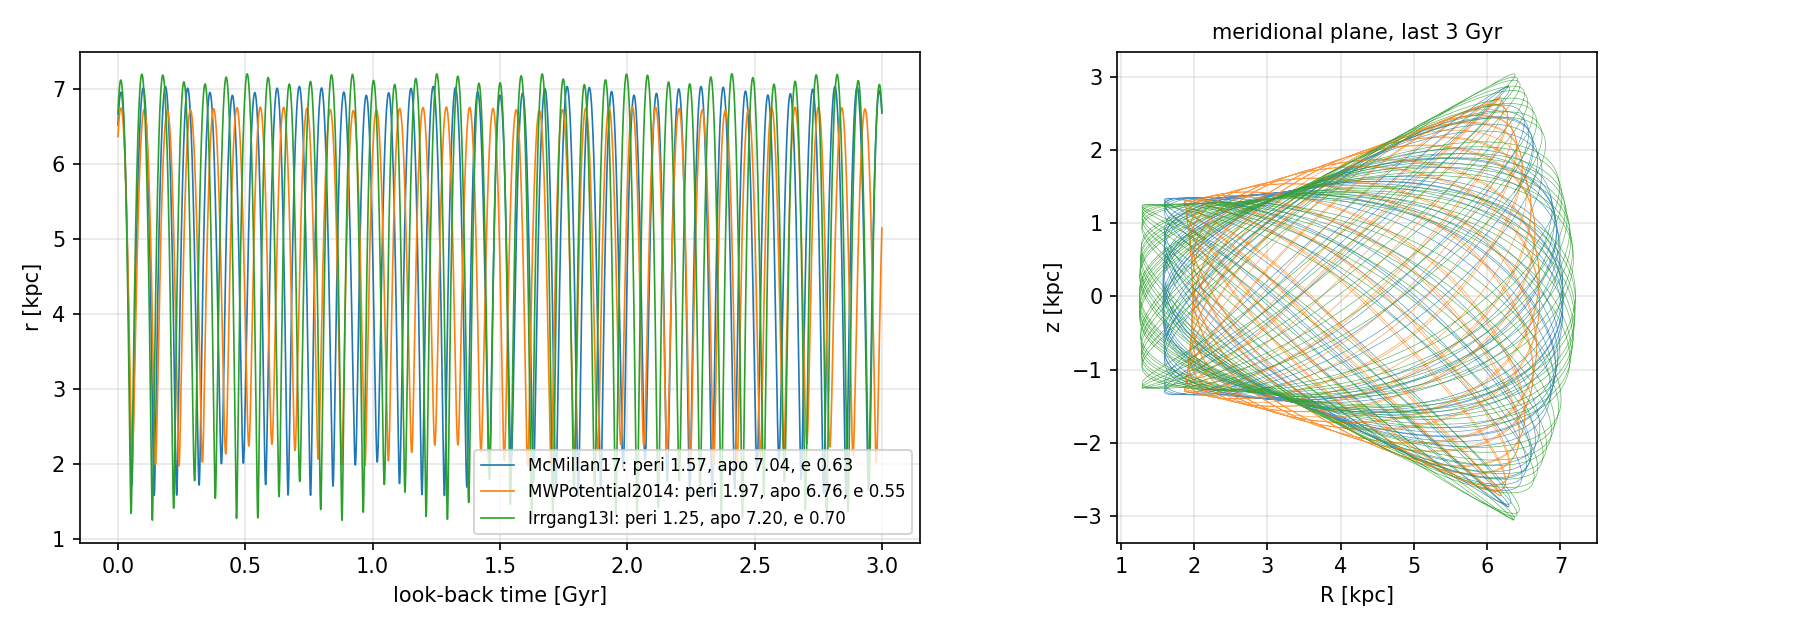
\includegraphics[width=\textwidth]{po_class1.png}
\caption{Class 1. Left: galactocentric radius over the last 3\,Gyr in the three potentials.
Right: the same orbits in the meridional plane. The orbit is a thick, eccentric, retrograde
loop confined to $z<3$\,kpc.}
\label{fig:c1}
\end{figure}

\section{Class 2: today's orbit with dynamical friction integrated backwards}

\subsection{Construction}
The equation of motion is integrated backwards in time with the Chandrasekhar deceleration
\citep{chandrasekhar1943} added,
\begin{equation}
\mathbf a_{\rm df} = -4\pi G^2 M(t)\,\rho(r)\,\ln\Lambda\,
\left[\mathrm{erf}(X)-\frac{2X}{\sqrt\pi}e^{-X^2}\right]\frac{\mathbf v}{v^3},
\qquad X=\frac{v}{\sqrt2\,\sigma},\quad \sigma=\frac{v_{\rm c}(r)}{\sqrt2},
\quad \ln\Lambda=\ln\frac{r}{\max(r_{\rm h},\,GM/v^2)} ,
\end{equation}
which is \texttt{galpy}'s prescription with its default Coulomb logarithm. Reversing time
reverses the sign of the friction term, so the orbit is pumped outwards: the integration
recovers where a satellite of bound mass $M(t)$ must have been to sink to the present orbit.
The host is McMillan (2017) evaluated with AGAMA \citep{vasiliev2019}; the integrator is a
leapfrog with 0.25\,Myr steps (about 1\,s per 10\,Gyr orbit). The frictionless run reproduces
class~1 (1.63/7.04 versus 1.57/7.04\,kpc), and a constant-mass case checked against
\texttt{galpy}'s \texttt{ChandrasekharDynamicalFrictionForce} agrees to 3\% in pericentre and
apocentre (1.84/47.1 versus 1.79/46.0\,kpc; 1\,s versus 482\,s).

\subsection{Assumptions, and which one matters}
\label{sec:c2assump}
Friction scales with the satellite's bound mass, so the backward orbit depends on the
\emph{function} $M(t)$. Integrating with a constant mass is not a conservative simplification:
it is wrong in the direction that matters. A constant $10^{10}\,\Msun$ satellite is pumped to
40--140\,kpc within 10\,Gyr, i.e.\ it ``arrives'' from outside the virial radius although the
real object had already been stripped to a small fraction of that mass for most of its orbit
(Fig.~\ref{fig:c2}, right).

We therefore parametrise the history and let a physical requirement select it:
\begin{enumerate}
\item \textbf{Infall mass $M_{\rm inf}$.} The nuclear-cluster--host relation gives
  $M_\star\approx10^9\,\Msun$ for the host \citep{pfeffer2021}; oMEGACat~X quotes a
  ``GE-like'' dwarf mass $4.5^{+5.7}_{-2.4}\times10^9\,\Msun$ and favours Sequoia/Thamnos over
  GSE as the debris \citep{souza2026}. Halo masses for $M_\star=10^8$--$10^9\,\Msun$ at
  $z\sim2$ are $10^{10}$--$10^{11}\,\Msun$; GSE itself is $2\times10^{11}\,\Msun$
  \citep{naidu2021}. Scanned: $10^{10},\,3\times10^{10},\,10^{11},\,2\times10^{11}\,\Msun$.
\item \textbf{Infall time} $t_{\rm inf}=10$\,Gyr ago ($z\approx2$; the GE merger is dated
  8--11\,Gyr ago). Also scanned 8\,Gyr; same conclusions.
\item \textbf{Stripping law} $M(t)=M_{\rm inf}\exp[-(t_{\rm inf}-t_{\rm lb})/\tau]$, floored
  at the nucleus mass $3.55\times10^6\,\Msun$ \citep{baumgardt2018}; $\tau$ scanned
  0.5--3\,Gyr. Half-mass radius $r_{\rm h}=1\,{\rm kpc}\,(M_{\rm inf}/10^{10}\,\Msun)^{1/3}$,
  fixed.
\item \textbf{Selection rule.} The orbit must be at the virial radius of the young Milky Way,
  50--150\,kpc, at $t_{\rm inf}$. Histories that do not reach 50\,kpc could not have sunk to
  today's orbit by friction alone; histories beyond 150\,kpc would need more friction than the
  mass allows.
\end{enumerate}

\subsection{Scan and picks}
Figure~\ref{fig:c2scan} shows the apocentre in the last Gyr before infall over the
$(M_{\rm inf},\tau)$ grid. The table is noisy at the 20\% level because the phase of the last
apocentre matters, but the trends are clear: a Sequoia-scale $10^{10}\,\Msun$ halo reaches the
virial radius only with slow stripping ($\tau\gtrsim1.5$\,Gyr); a GSE-scale halo must be
stripped fast ($\tau\lesssim1$\,Gyr) or it arrives from far outside the virial radius. Three
histories spanning the allowed band are kept (Table~\ref{tab:c2}). In every viable history the
bound mass is below $10^9\,\Msun$ by 5\,Gyr ago and the orbit has today's shape for the last
3--5\,Gyr (Fig.~\ref{fig:c2}, middle): \emph{the present orbit is a good proxy for the second
half of the history in all cases}, and the classes differ in the first half.

\begin{table}[h]\centering
\caption{Class-2 picks (kpc). Columns 5--6: pericentre--apocentre range in the stated
look-back window.}
\label{tab:c2}
\begin{tabular}{lcccccc}\toprule
label & $M_{\rm inf}$ [$\Msun$] & $\tau$ [Gyr] & $r$ at infall & 5--6\,Gyr ago & 2--3\,Gyr ago\\\midrule
Sequoia-like & $10^{10}$ & 2.0 & 65 & 2.9--17.9 & 2.0--9.2\\
intermediate & $3\times10^{10}$ & 1.25 & 85 & 2.2--11.6 & 1.7--7.4\\
GSE-like & $10^{11}$ & 0.75 & 111 & 1.7--7.5 & 1.6--7.1\\
\bottomrule\end{tabular}
\end{table}

\begin{figure}[h]\centering
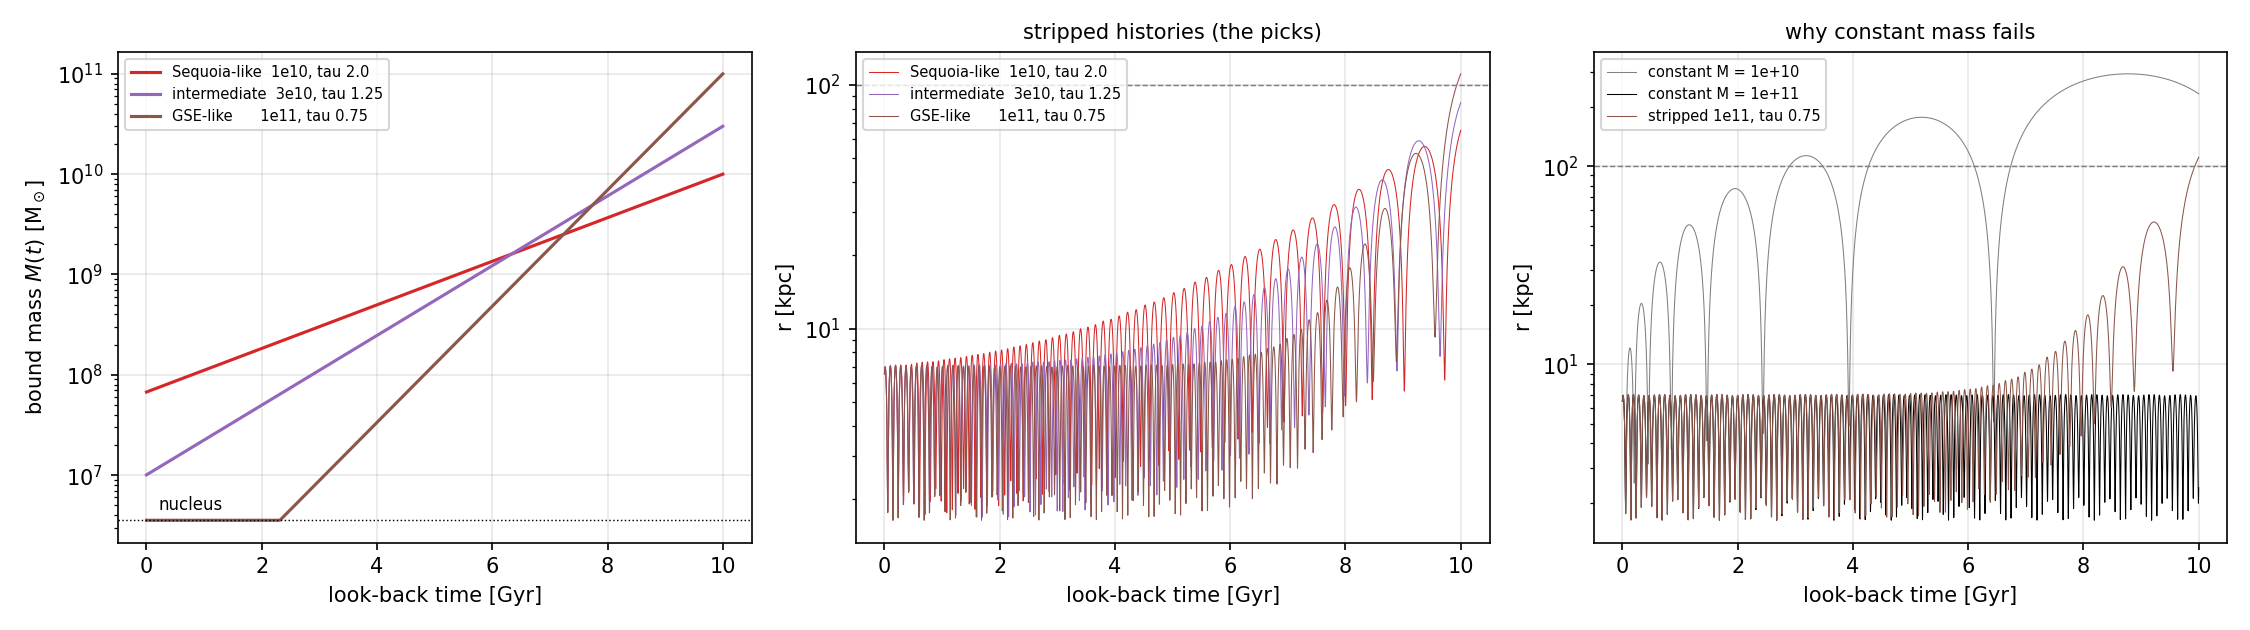
\includegraphics[width=\textwidth]{po_class2.png}
\caption{Class 2. Left: the three adopted bound-mass histories. Middle: the corresponding
backward orbits; the dashed line marks 100\,kpc. Right: why a constant mass fails --- a
constant $10^{10}\,\Msun$ satellite (grey) is pumped beyond the virial radius within
10\,Gyr, a constant $10^{11}\,\Msun$ one (black) escapes even faster, while the stripped
$10^{11}$ history (brown) stays on today's orbit for 6\,Gyr and arrives from 110\,kpc.}
\label{fig:c2}
\end{figure}

\begin{figure}[h]\centering
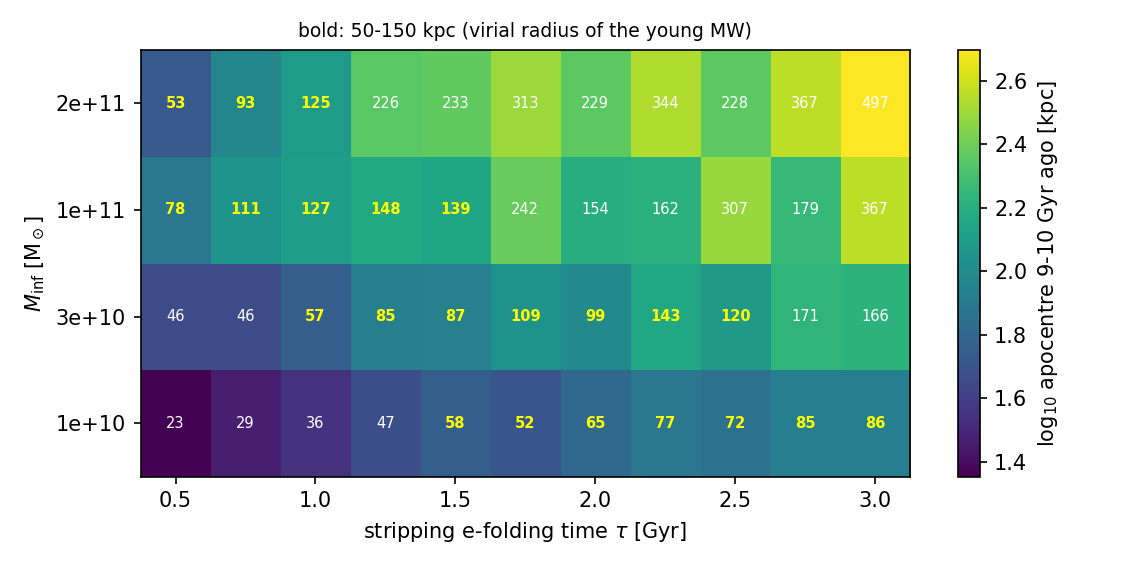
\includegraphics[width=0.8\textwidth]{po_class2_scan.png}
\caption{Class 2: apocentre 9--10\,Gyr ago as a function of infall mass and stripping
e-folding time ($t_{\rm inf}=10$\,Gyr). Bold entries satisfy the 50--150\,kpc selection
rule. Low-mass halos need slow stripping, GSE-mass halos fast stripping.}
\label{fig:c2scan}
\end{figure}

\section{Class 3: deposited by GSE, migrated inward by the bar}

\subsection{What the literature provides}
\citet{dillamore2026} showed that \ocen\ can be traced back to the GSE debris region of
$(\Lz,E)$ if the Galactic bar has decelerated and its present pattern speed is
$\Ob\lesssim26$\,\kmskpc, well below most current estimates. The mechanism is the retrograde
1:1 resonance, $\Omega_\phi-\Ob+\Omega_r=0$, which scatters orbits to lower $E$ and more
retrograde $\Lz$. Friction on the nucleus is negligible ($\dot\Lz\approx9.6$\,kpc\,\kms\,Gyr$^{-1}$).
The GSE debris itself is characterised by \citet{belokurov2023}: $|\Lz|<700$\,kpc\,\kms,
chevrons with apocentres 11.5--25\,kpc, and a set of $(\Lz,E)$ contours that we use directly.

\subsection{Construction: reproducing the published set-up}
The authors' pipeline (repository \texttt{adllmr/oCen\_bar}, local clone
\texttt{$\sim$/Work/Code/oCen\_bar}) was followed step by step; its potential files and contour
file are referenced, not copied.
\begin{itemize}
\item \textbf{Potential.} \citet{hunter2024} Milky Way with the \citet{sormani2022} bar
  ($M_{\rm bar}=1.83\times10^{10}\,\Msun$), as AGAMA files. The model is decomposed as
  $\Phi=\Phi_{\rm axi}+A(t)\,\Phi_{\rm bar}[S(t)]-A(t)\,\bar\Phi_{\rm bar}[S(t)]$, i.e.\ the
  axisymmetric total plus the scaled, rotating baryonic bar part minus the same part
  azimuthally averaged, so the $m=0$ mass is unchanged while the bar grows.
\item \textbf{Bar history.} Amplitude $A$ follows the \citet{dehnen2000} switch-on between
  $t=0$ and $t_1=1$\,Gyr. The pattern speed is $\Omega_1$ until $t_1$, starts decelerating
  smoothly to $t_2=2$\,Gyr, then obeys $\eta\equiv-\dot\Ob/\Ob^2=0.003$ until
  $t_f=8$\,Gyr (the bar age). $\Omega_1$ is fixed by the present-day $\Ob$:
  $\Omega_1=45.1$\,\kmskpc\ for $\Ob=24$ (the paper quotes ``$\approx45$'', which confirms
  $t_1,t_2=1,2$\,Gyr rather than the 2,\,3 defaults left in one of the repository functions),
  72 for 30, 110 for 35. The bar length scales as $S(t)=\Ob(t_f)/\Ob(t)$, approximately the
  corotation radius, at fixed amplitude (Fig.~\ref{fig:c3bar}, left).
\item \textbf{Samples.} $N=10^3$ draws of the present-day state (Sec.~\ref{sec:present}),
  bar angle $28^\circ$, integrated from $t_f$ back to 0 with \texttt{agama.orbit}.
\item \textbf{Test.} $(E,\Lz)$ at $t=0$ in the axisymmetric potential, compared with the
  outermost \citet{belokurov2023} contour after matching the energy zero point at
  $R=8.2$\,kpc. Our success metric is the fraction of samples inside that contour.
\end{itemize}

\subsection{Results}
\begin{table}[h]\centering
\caption{Fraction of the $10^3$ samples inside the outer GSE contour 8\,Gyr ago.}
\label{tab:c3grid}
\begin{tabular}{l*{13}{c}}\toprule
$\Ob$ [\kmskpc] & 20 & 21 & 22 & 22.5 & 23 & 23.5 & 24 & 24.5 & 25 & 25.5 & 26 & 26.5 & $\ge27$\\\midrule
fraction & 0.44 & 0.38 & 0.58 & 0.85 & 0.01 & 0.34 & \textbf{0.89} & 0.81 & 0.79 & 0.54 & 0.18 & 0.02 & 0.00\\
\bottomrule\end{tabular}
\end{table}

\begin{itemize}
\item The published result is reproduced: overlap with GSE only for $\Ob\lesssim26$, none for
  the mainstream 30--40\,\kmskpc\ (Fig.~\ref{fig:c3elz}).
\item Cross-check against the authors' stored grid (\texttt{oCen\_bar/artifacts/03\_orbit\_grid.npz}):
  0.87, 0.69, 0.08 at $\Ob=24,25,26$ with a dip at 23 --- the same pattern. The dip is stable
  against the random seed (0.013 versus 0.028) and against the bar timings: it is
  resonant-phase sensitivity, not noise. The $\Ob$ dependence is intrinsically jagged.
\item \textbf{Migration is late.} $E$ and $\Lz$ of the successful samples stay at GSE-like
  values from 8 to $\sim$2.5\,Gyr ago and move to today's values only in the last
  $\sim$2.5\,Gyr, while $\Ob$ falls from $\sim$30 to 24 and the resonance sweeps across \ocen\
  (Fig.~\ref{fig:c3picks}). The pre-migration $\Lz$ is \emph{slightly prograde to zero}
  ($+70$ to $+230$\,kpc\,\kms), not retrograde.
\item \textbf{The bar changes today's orbit.} At $\Ob=24$ corotation is at $\approx9.5$\,kpc,
  so \ocen\ at 6.5\,kpc is inside corotation. Its present orbit in the barred potential has
  peri/apo $=0.81/9.3$\,kpc over the last Gyr, versus $1.56/7.02$ in the axisymmetrised
  Hunter potential and $1.57/7.04$ in McMillan 2017. ``Today's orbit'' in class~1 is therefore
  conditional on the bar being fast or absent.
\end{itemize}

\begin{table}[h]\centering
\caption{Class-3 picks at $\Ob=24$: samples at the 16/50/84th percentiles of $E(t=0)$ among
those ending inside GSE. Elements from a 0.25-Myr re-integration (the 20-Myr grid cadence
overestimates pericentres by up to a factor 2, since a passage at 0.4\,kpc lasts $\sim$1\,Myr).}
\label{tab:c3picks}
\begin{tabular}{lcccc}\toprule
sample & $E(0)$ [$10^5$] & $\Lz(0)$ & pre-migration peri/apo/$e$/$z_{\max}$ (7--8\,Gyr ago) & last Gyr peri/apo\\\midrule
986 & $-1.301$ & $+69$ & 0.40 / 10.9 / 0.93 / 4.8 & 0.84 / 9.1\\
133 & $-1.265$ & $+163$ & 0.42 / 11.6 / 0.93 / 4.9 & 0.80 / 9.3\\
240 & $-1.233$ & $+229$ & 0.45 / 12.2 / 0.93 / 5.2 & 0.84 / 9.1\\
\bottomrule\end{tabular}
\end{table}

\begin{figure}[p]\centering
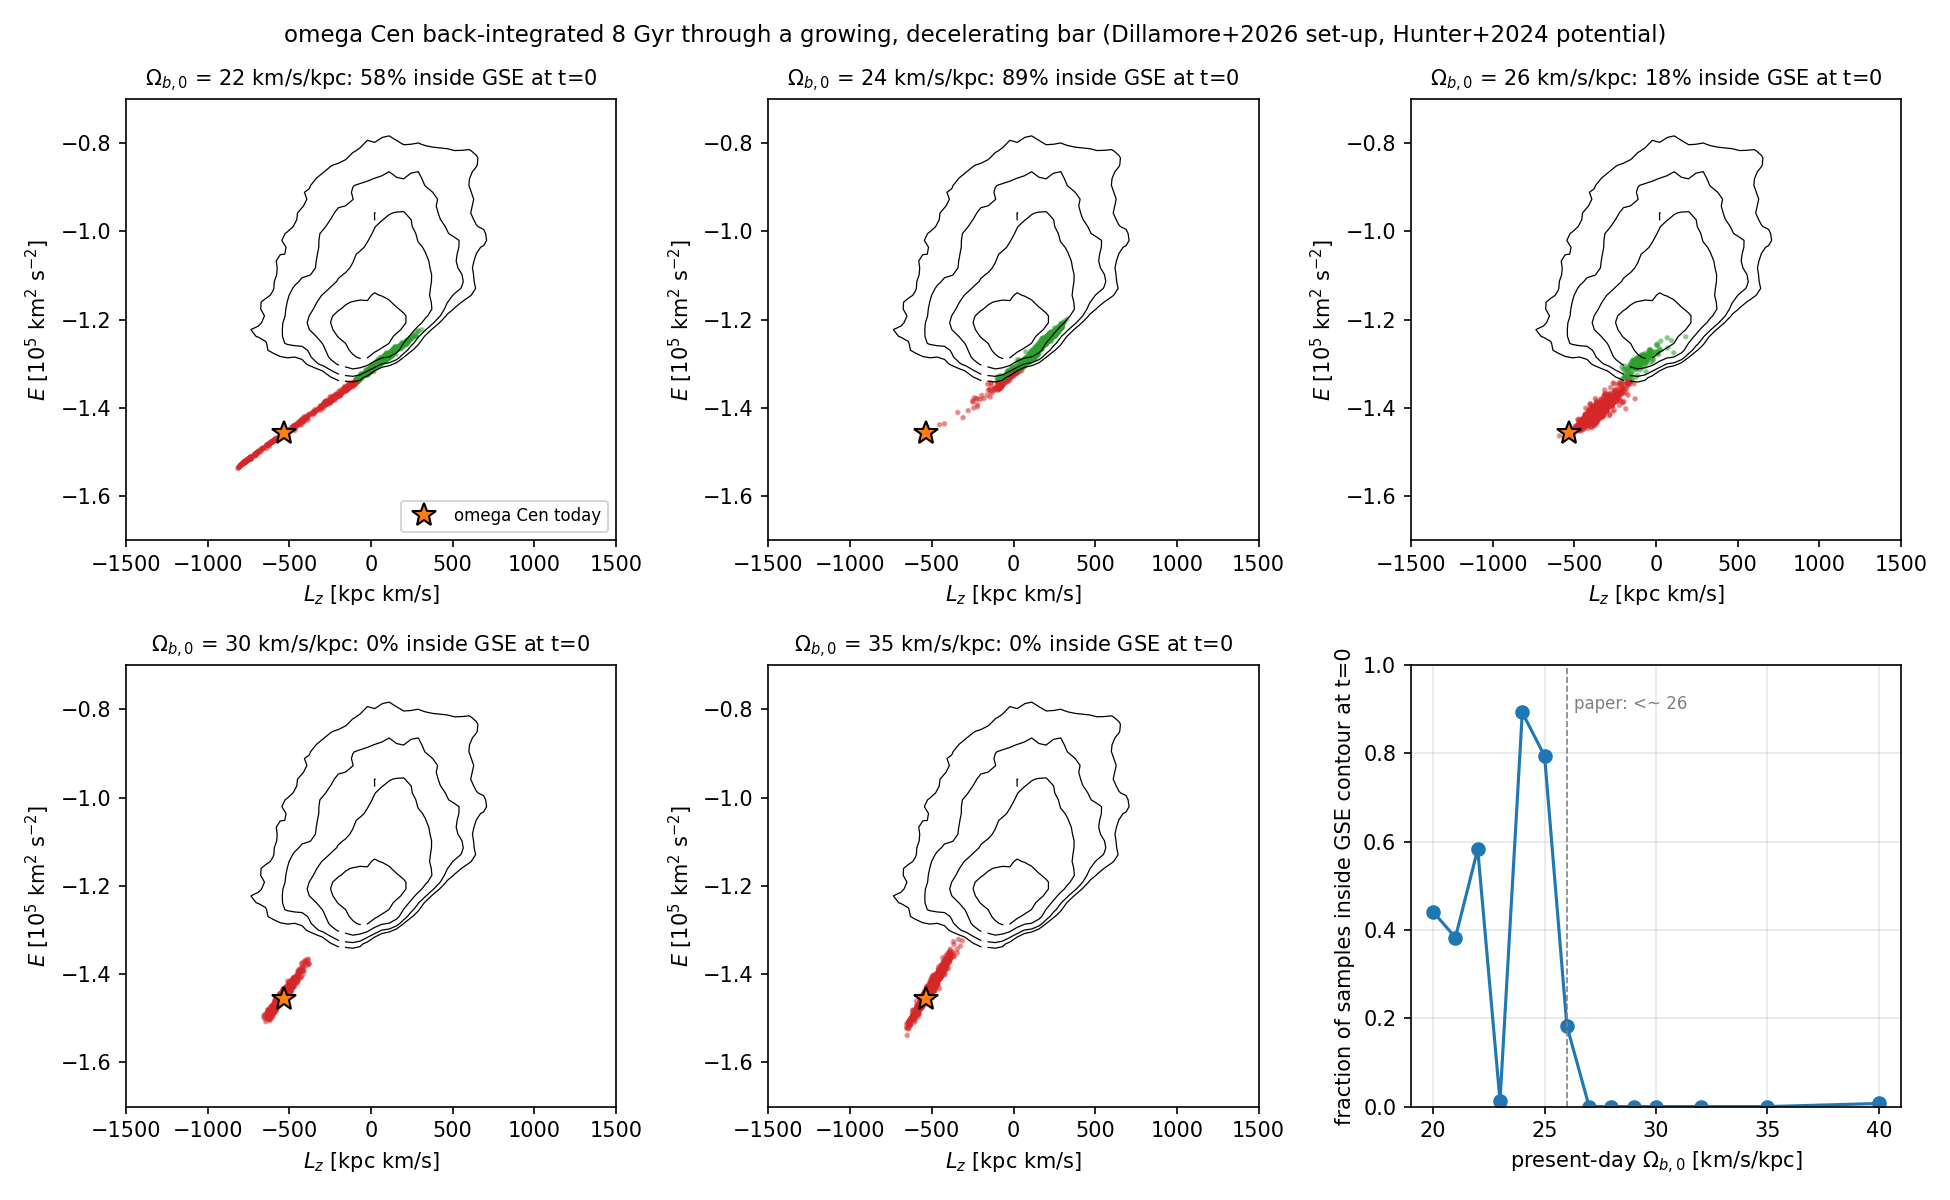
\includegraphics[width=\textwidth]{bar_migration_elz.png}
\caption{Class 3, the $(\Lz,E)$ plane in the axisymmetrised Hunter et al.\ (2024) potential.
Black: GSE contours of Belokurov et al.\ (2023). Star: \ocen\ today. Points: the $10^3$
samples 8\,Gyr ago after back-integration through the decelerating bar, green inside / red
outside the outer contour. Bottom right: fraction inside versus present-day pattern speed;
the dashed line is the paper's $\Ob\lesssim26$.}
\label{fig:c3elz}
\end{figure}

\begin{figure}[p]\centering
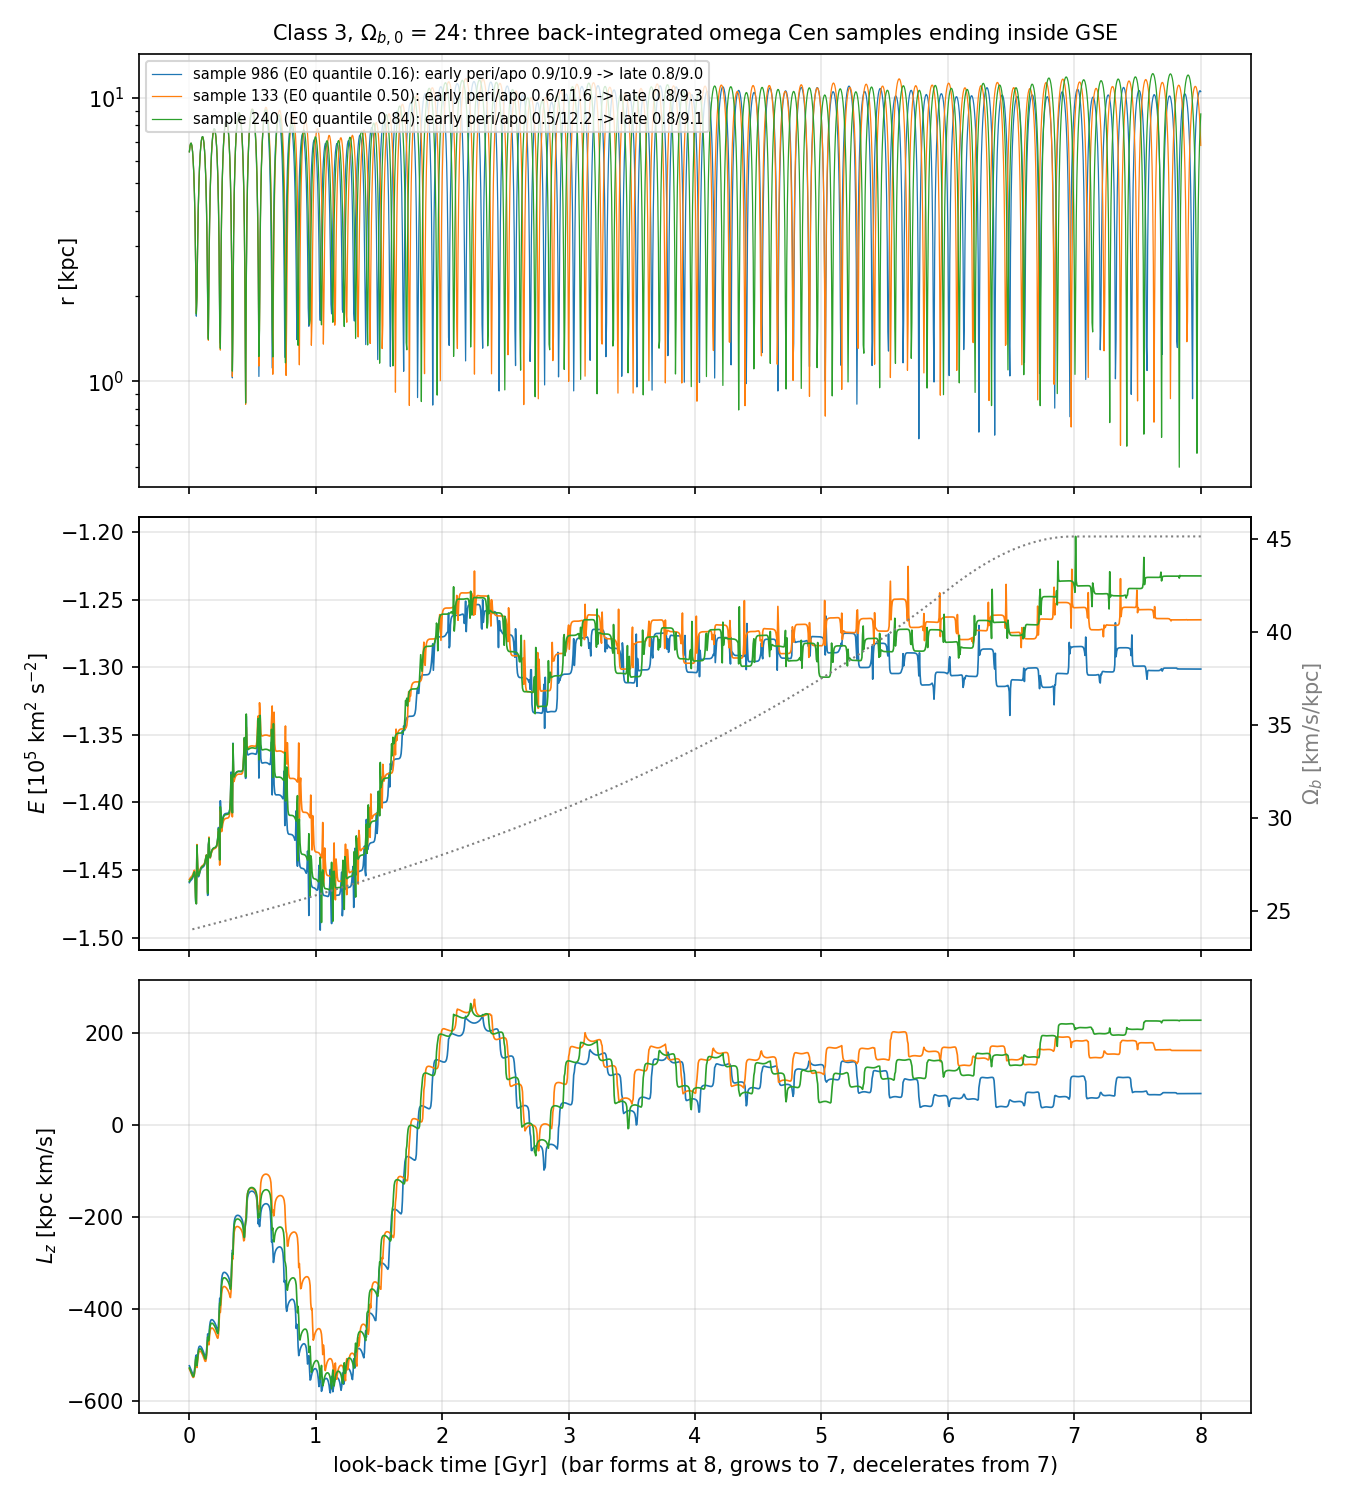
\includegraphics[width=0.9\textwidth]{bar_migration_class3_picks.png}
\caption{Class 3, the three picked samples at $\Ob=24$: radius, energy (dotted grey: $\Ob(t)$)
and $\Lz$ against look-back time. The bar forms 8\,Gyr ago and grows until 7; the nucleus sits
on a GSE-debris orbit until $\sim$2.5\,Gyr ago and is then carried to today's $(E,\Lz)$ by the
retrograde 1:1 resonance. Look-back time here is $t_f-t$.}
\label{fig:c3picks}
\end{figure}

\begin{figure}[h]\centering
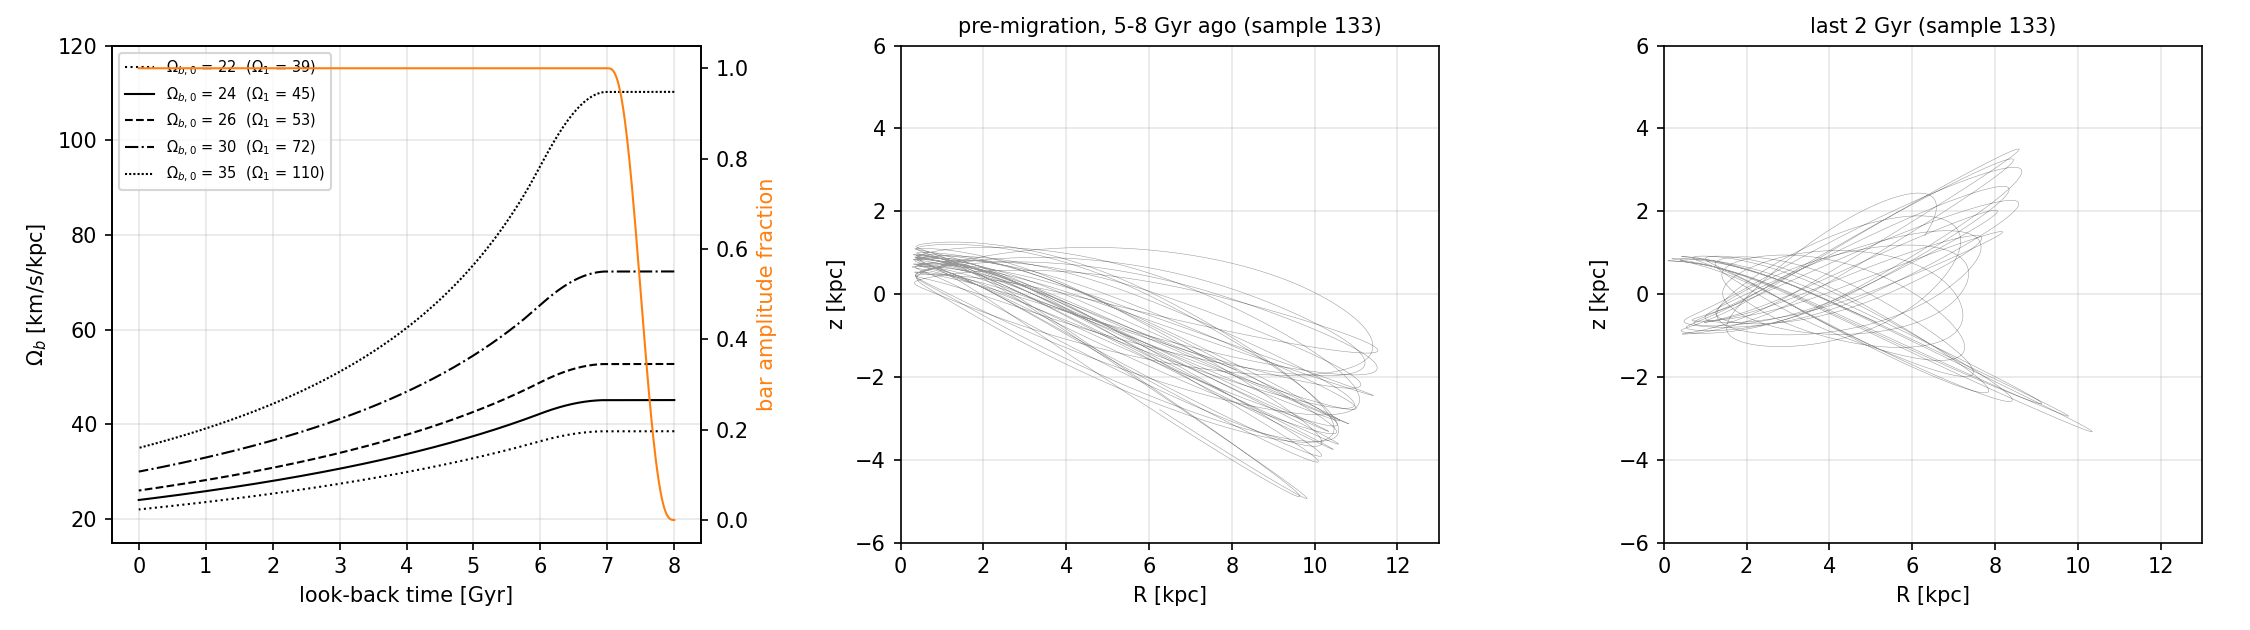
\includegraphics[width=\textwidth]{po_class3_bar.png}
\caption{Class 3. Left: pattern-speed histories for several present-day values (black) and
the bar amplitude switch-on (orange, right axis); with fixed $\eta=0.003$ a present-day
$\Ob=35$ demands an initial $\Omega_1=110$\,\kmskpc. Middle and right: the median pick
(sample 133) in the meridional plane before migration and in the last 2\,Gyr --- a plunging,
highly inclined debris orbit turning into a rounder, lower orbit.}
\label{fig:c3bar}
\end{figure}

\subsection{What is still not modelled in class 3}
Anything before the bar formed ($>8$\,Gyr ago): GSE's own infall and disruption
\citep[fiducial: $M_\star=5\times10^8$, $M_{\rm DM}=2\times10^{11}\,\Msun$, $c=4$, from
$R_{\rm vir}$ at $z\approx2$, circularity 0.5, retrograde;][]{naidu2021} and where \ocen's
host sat in it. Two readings of ``deposited by GSE'' remain open --- \ocen\ is GSE's own nucleus
\citep{pfeffer2021}, or its host was a smaller dwarf that fell in with GSE (group infall, the
oMEGACat~X reading) --- and both start the disruption on the picked debris orbit. The bar
history is a one-parameter family at fixed $\eta$; the oCen\_bar journal notes that the
low-$\Ob$ requirement is tied to this slowdown law, since $\Ob=35$ today implies an
implausible $\Omega_1=110$\,\kmskpc.

\section{Comparison between the classes}

\begin{figure}[p]\centering

\includegraphics[width=\textwidth]{progenitor_orbits.png}
\caption{Overview of the nine orbits: galactocentric radius against look-back time for classes
1 (top), 2 (middle; dashed line 100\,kpc) and 3 (bottom). Dotted line: today's apocentre,
7\,kpc.}
\label{fig:overview}
\end{figure}

\begin{figure}[p]\centering
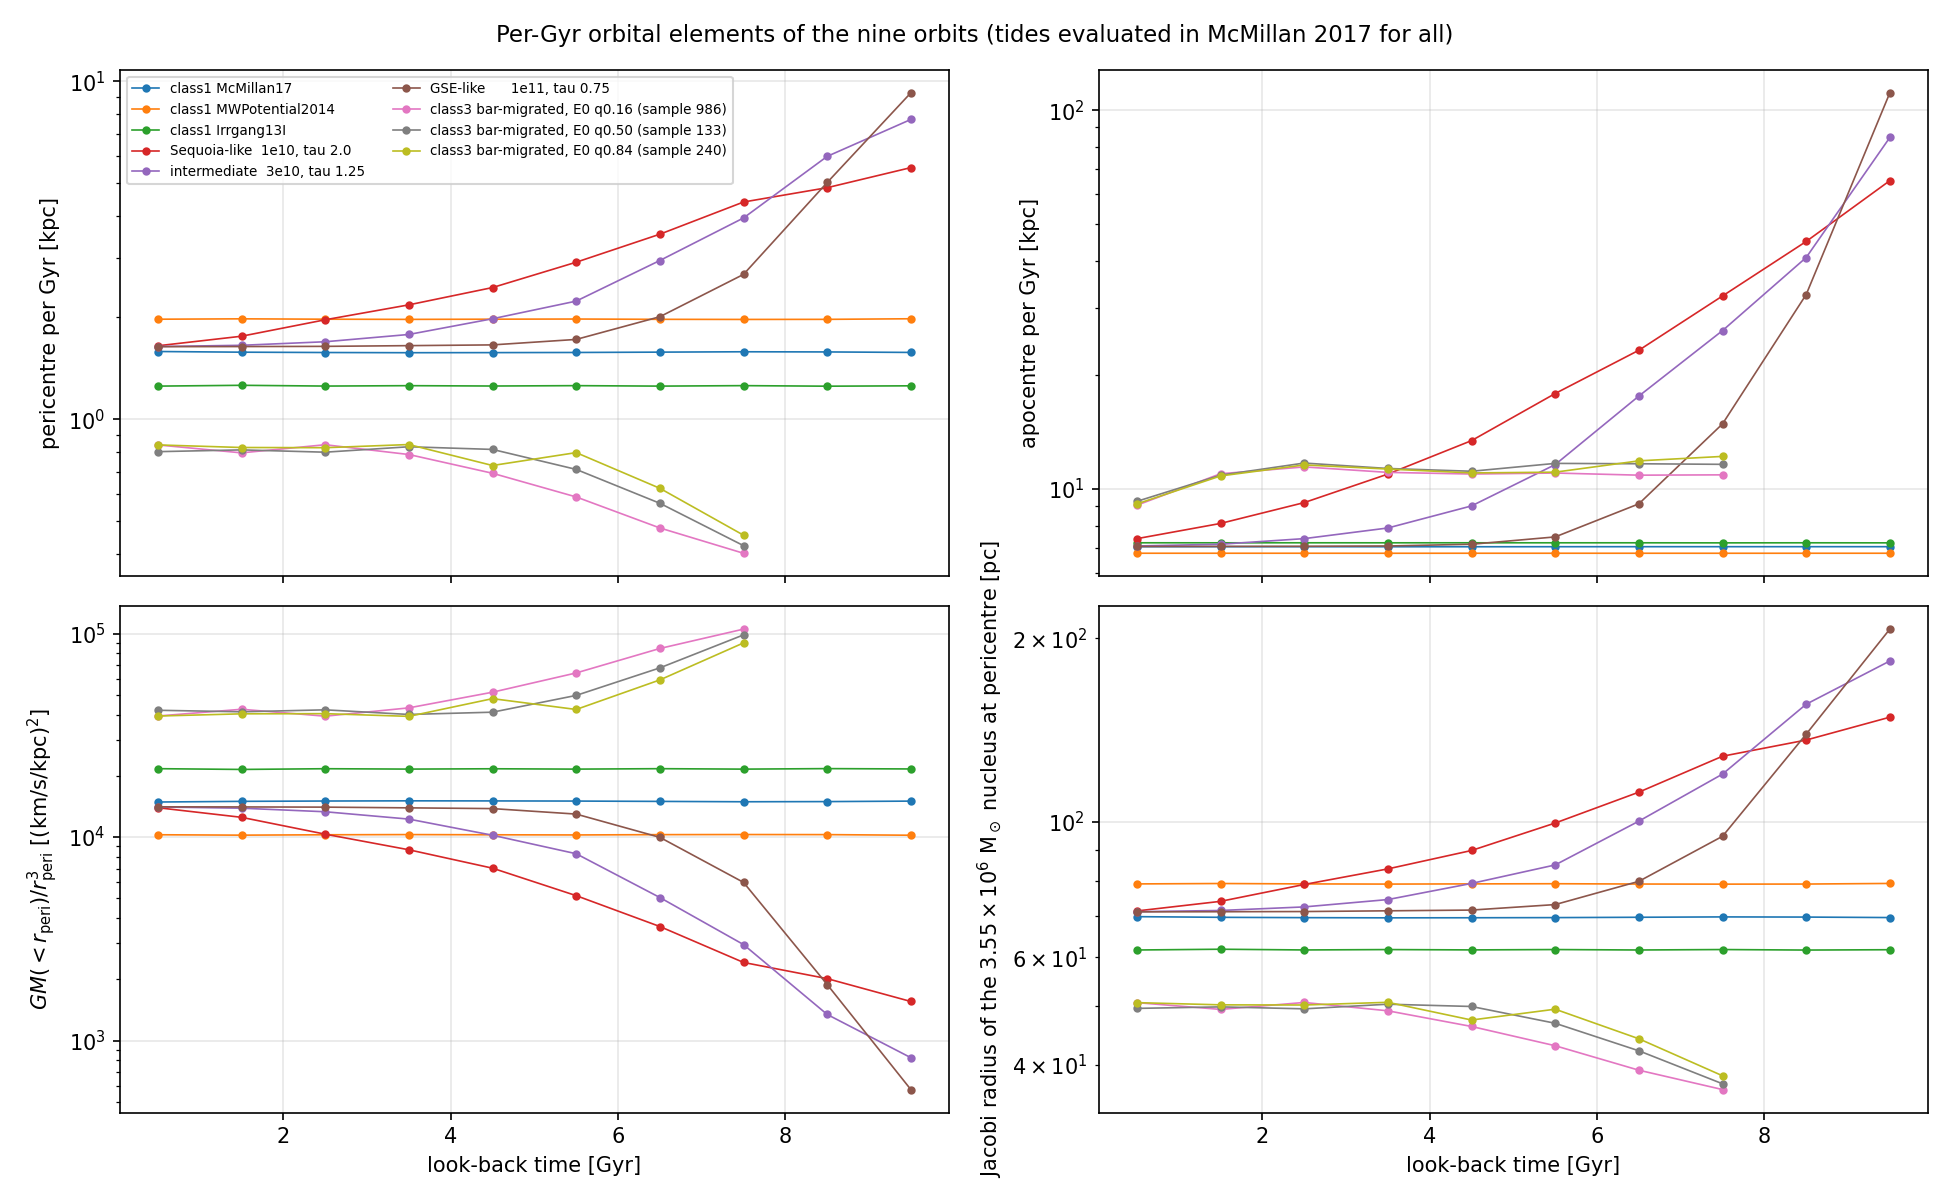
\includegraphics[width=\textwidth]{po_comparison.png}
\caption{Per-Gyr orbital elements of the nine orbits: pericentre, apocentre, tidal-field
strength $GM(<r_{\rm peri})/r_{\rm peri}^3$ at pericentre, and the Jacobi radius a
$3.55\times10^6\,\Msun$ nucleus would have there. Enclosed masses from McMillan (2017) for all
orbits, including class 3 (integrated in Hunter et al.\ 2024), for a uniform proxy.}
\label{fig:comparison}
\end{figure}

\begin{figure}[h]\centering
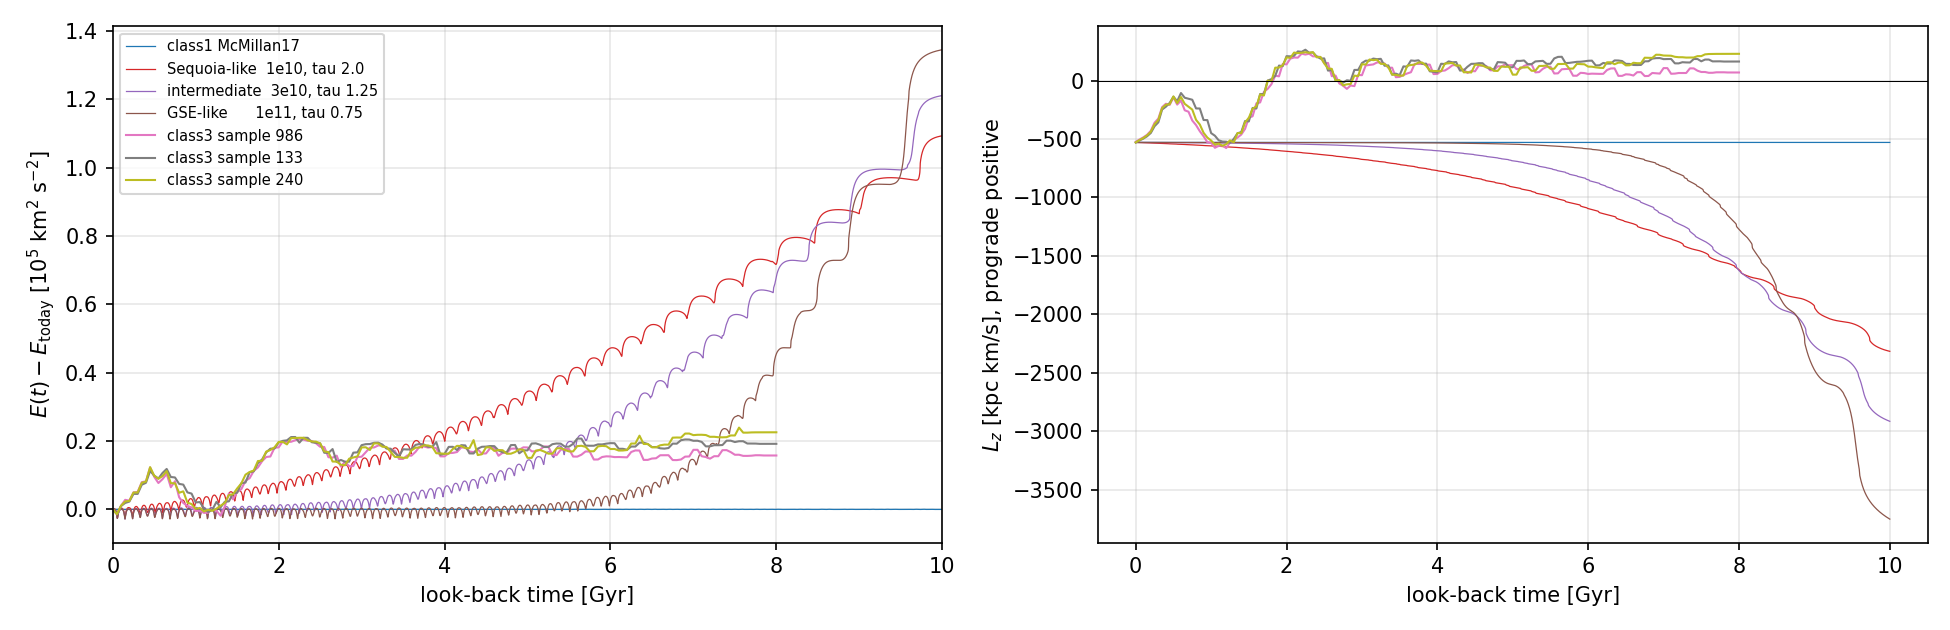
\includegraphics[width=\textwidth]{po_E_Lz.png}
\caption{Energy relative to today (left; each orbit in its own host potential) and $\Lz$
(right, prograde-positive) against look-back time. Class 1 (McMillan 2017 only) is flat by
construction; class 2 climbs steadily as friction is undone; class 3 is flat at GSE values
until the resonance moves it in the last 2.5\,Gyr. Note the opposite directions of the $\Lz$
change: friction makes the early orbit \emph{more} retrograde, the bar makes it \emph{less}.}
\label{fig:elz}
\end{figure}

Figure~\ref{fig:comparison} and Table~\ref{tab:cmp} summarise what a disruption simulation
would see.

\begin{table}[h]\centering
\caption{Per-Gyr elements at three epochs (kpc unless stated). Tidal strength $T\equiv
GM(<r_{\rm peri})/r_{\rm peri}^3$ in $10^3$\,(\kms/kpc)$^2$; $r_J$ is the Jacobi radius of a
$10^9\,\Msun$ host at pericentre in the last Gyr.}
\label{tab:cmp}
\begin{tabular}{llcccccc}\toprule
class & orbit & peri (0--1 / 5--6 / 8--9\,Gyr) & apo (0--1 / 5--6 / 8--9) & $T$ (0--1) & $T$ (8--9) & $r_J^{10^9}$\\\midrule
1 & McMillan 2017 & 1.59 / 1.58 / 1.58 & 7.0 / 7.0 / 7.0 & 14.9 & 14.9 & 0.46\\
1 & MWPotential2014 & 1.98 / 1.98 / 1.97 & 6.8 / 6.8 / 6.8 & 10.3 & 10.3 & 0.52\\
1 & Irrgang 2013 I & 1.25 / 1.26 / 1.25 & 7.2 / 7.2 / 7.2 & 21.7 & 21.7 & 0.40\\
2 & Sequoia-like & 1.65 / 2.91 / 4.84 & 7.4 / 17.9 / 45 & 13.9 & 1.9 & 0.47\\
2 & intermediate & 1.64 / 2.24 / 5.99 & 7.1 / 11.6 / 41 & 14.1 & 1.4 & 0.47\\
2 & GSE-like & 1.64 / 1.72 / 5.01 & 7.0 / 7.5 / 33 & 14.1 & 1.9 & 0.47\\
3 & sample 986 & 0.84 / 0.59 / 0.40 & 9.1 / 11.0 / 10.9 & 39.4 & 104 & 0.33\\
3 & sample 133 & 0.80 / 0.71 / 0.42 & 9.3 / 11.7 / 11.6 & 42.0 & 100 & 0.32\\
3 & sample 240 & 0.84 / 0.80 / 0.45 & 9.1 / 11.1 / 12.2 & 39.4 & 92 & 0.33\\
\bottomrule\end{tabular}
\end{table}

\paragraph{Late history (last 3\,Gyr).} Classes 1 and 2 are indistinguishable: pericentre
1.6\,kpc, apocentre 7\,kpc, $T\approx1.4\times10^4$\,(\kms/kpc)$^2$. Class 3 is different even
today because the slow bar is part of its potential: pericentre 0.8\,kpc and three times
stronger pericentric tides. Whether that is a property of class~3 or of the Galaxy depends
only on whether the bar is slow; if it is, classes 1 and 2 should be re-evaluated in the
barred potential as well.

\paragraph{Early history (5--10\,Gyr ago).} This is where the classes separate, by more than an
order of magnitude in tidal strength. Class 1 keeps today's tides throughout. Class 2 has a
gentle early history: pericentres of 2--6\,kpc and $T$ ten times weaker than today, so the host
is stripped slowly at first and hardest at the end, when it is already light. Class 3 is the
opposite: pericentres of 0.4\,kpc through the bulge with $T$ seven times \emph{stronger} than
today and a Jacobi radius of only 0.3\,kpc for a $10^9\,\Msun$ host --- the host is destroyed
early and violently, and what survives to be migrated by the bar is the nucleus alone. For
the dark-matter question this is the sharpest distinction: a class-3 history leaves the
nucleus the least time to retain a dark envelope, a class-2 history the most.

\paragraph{Angular momentum.} The early orbit is more retrograde than today in class 2
($\Lz\to-2000$ to $-4000$\,kpc\,\kms\ as friction is undone) and \emph{less} retrograde in
class 3 ($\Lz\approx0$ to $+230$; Fig.~\ref{fig:elz}). Retrograde class-2 infall is consistent
with the retrograde Sequoia/Thamnos association; a class-3 host arrives on the near-radial GSE
orbit.

\paragraph{Robustness.} Class 1 depends only on the potential (factor 1.6 in pericentre).
Class 2 depends on $M(t)$ far more than on any single mass, and the selection rule of
Sec.~\ref{sec:c2assump} is what makes the set finite; the friction formula itself is a
20--30\% approximation. Class 3 depends on the bar's slowdown law and on a present-day pattern
speed at the low end of the literature, and its success is a jagged function of $\Ob$.

\section{Caveats and reproducibility}
\begin{itemize}
\item Chandrasekhar friction with $\sigma=v_{\rm c}/\sqrt2$, a fixed $r_{\rm h}$ and a
  smooth exponential stripping law; no orbit-phase-dependent mass loss.
\item Only McMillan (2017) for class 2; only Hunter et al.\ (2024) for class 3 (the only
  potential with a fitted bar); class 1 carries the potential spread.
\item Tidal proxies in Fig.~\ref{fig:comparison} use McMillan (2017) enclosed masses for all
  classes.
\item The \texttt{galpy} checkout used (2024-03) needs two import shims (astroquery metadata,
  scipy \texttt{vectorize1}); both live in \texttt{progenitor\_orbits.\_import\_galpy\_safely}.
\item Products: \texttt{python -m ocen\_dm.tails.products}, \texttt{python -m ocen\_dm.tails.bar\_migration},
  \texttt{python -m ocen\_dm.tails.writeup\_figures}. The class-3 run of $14\times10^3$ orbits
  takes about a minute.
\end{itemize}

\clearpage
\begin{thebibliography}{99}
\bibitem[Baumgardt \& Hilker(2018)]{baumgardt2018} Baumgardt, H., Hilker, M. 2018, MNRAS, 478, 1520, \url{https://doi.org/10.1093/mnras/sty1057}
\bibitem[Baumgardt \& Vasiliev(2021)]{baumgardt2021} Baumgardt, H., Vasiliev, E. 2021, MNRAS, 505, 5957, \url{https://doi.org/10.1093/mnras/stab1474}
\bibitem[Belokurov et al.(2023)]{belokurov2023} Belokurov, V., Vasiliev, E., Deason, A. J., et al. 2023, MNRAS, 518, 6200, \url{https://arxiv.org/abs/2208.11135}
\bibitem[Bovy(2015)]{bovy2015} Bovy, J. 2015, ApJS, 216, 29, \url{https://doi.org/10.1088/0067-0049/216/2/29}
\bibitem[Chandrasekhar(1943)]{chandrasekhar1943} Chandrasekhar, S. 1943, ApJ, 97, 255, \url{https://doi.org/10.1086/144517}
\bibitem[Dehnen(2000)]{dehnen2000} Dehnen, W. 2000, AJ, 119, 800, \url{https://doi.org/10.1086/301226}
\bibitem[Dillamore et al.(2026)]{dillamore2026} Dillamore, A. M., Zhang, H., Belokurov, V. 2026, arXiv:2606.12516, \url{https://arxiv.org/abs/2606.12516}
\bibitem[Hunter et al.(2024)]{hunter2024} Hunter, G. H., Sormani, M. C., Beckmann, J. P., et al. 2024, A\&A, 692, A216, \url{https://www.aanda.org/articles/aa/pdf/2024/12/aa50000-24.pdf}
\bibitem[Irrgang et al.(2013)]{irrgang2013} Irrgang, A., Wilcox, B., Tucker, E., Schiefelbein, L. 2013, A\&A, 549, A137, \url{https://doi.org/10.1051/0004-6361/201220540}
\bibitem[McMillan(2017)]{mcmillan2017} McMillan, P. J. 2017, MNRAS, 465, 76, \url{https://doi.org/10.1093/mnras/stw2759}
\bibitem[Naidu et al.(2021)]{naidu2021} Naidu, R. P., Conroy, C., Bonaca, A., et al. 2021, ApJ, 923, 92, \url{https://arxiv.org/abs/2103.03251}
\bibitem[Pfeffer et al.(2021)]{pfeffer2021} Pfeffer, J., Lardo, C., Bastian, N., Saracino, S., Kamann, S. 2021, MNRAS, 500, 2514, \url{https://academic.oup.com/mnras/article/500/2/2514/5956542}
\bibitem[Sch\"onrich et al.(2010)]{schoenrich2010} Sch\"onrich, R., Binney, J., Dehnen, W. 2010, MNRAS, 403, 1829, \url{https://doi.org/10.1111/j.1365-2966.2010.16253.x}
\bibitem[Sormani et al.(2022)]{sormani2022} Sormani, M. C., Gerhard, O., Portail, M., Vasiliev, E., Clarke, J. 2022, MNRAS, 514, L1, \url{https://doi.org/10.1093/mnrasl/slac046}
\bibitem[Souza et al.(2026)]{souza2026} Souza, S. O., Neumayer, N., Seth, A. C., et al. 2026, arXiv:2603.23589, \url{https://arxiv.org/abs/2603.23589}
\bibitem[Vasiliev(2019)]{vasiliev2019} Vasiliev, E. 2019, MNRAS, 482, 1525, \url{https://doi.org/10.1093/mnras/sty2672}
\bibitem[Vasiliev \& Baumgardt(2021)]{vasiliev2021} Vasiliev, E., Baumgardt, H. 2021, MNRAS, 505, 5978, \url{https://doi.org/10.1093/mnras/stab1475}
\end{thebibliography}
\end{document}
